\subsection{Poly Etcher (DRY-Poly)}\label{poly_etcher_machine}
\WaferClean\WaferSemiClean

\begin{minipage}[H]{\MachinePictureMiniPageWidth}
	%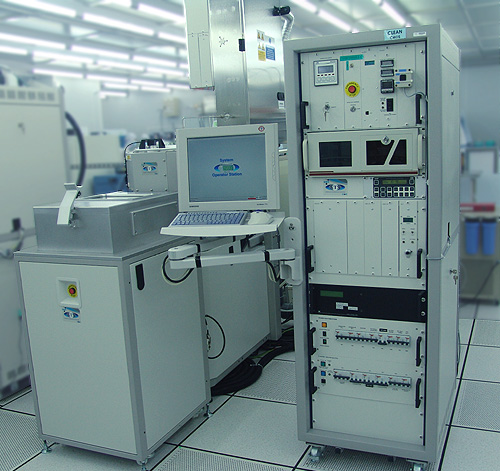
\includegraphics[width=\MachinePictureWidth]{pictures_machines/poly_etcher.png}
\end{minipage}\begin{minipage}[H]{\MachineTextMiniPageWidth}
	\begin{tabular}{|p{3cm}|p{8cm}|}
		\hline
		Remark &
		For Semi-Clean process, please contact NFF technicians. \\
		\hline
		Gases available &
		$H Br$, $Cl_2$, $O_2$, $N_2$, $He$ and $Ar$ \\
		\hline
		RF power source &
		\makecell[l]{
			\tabitem 1x 1000W(max) at 13.56MHz for Coil electrode \\
			\tabitem 1x 300W(max)  at 13.56MHz for Platen electrode
		} \\
		\hline
		Electrode coolant system &
		20 \degreesC \\
		\hline
		High speed turbo molecular pump &
		\makecell[l]{
			\tabitem Pumping speed of 1000 L/s at 36000 rpm \\
			\tabitem Fully automatic loadlock transfer system
		} \\
		\hline
		Substrate size &
		4” single wafer \\
		\hline
	\end{tabular}

	\underline{Polysilicon etch}

	\begin{tabular}{|p{5cm}|p{6cm}|}
		\hline
		Minimum line/space &
		0.5\um \\
		\hline
		Low rate polysilicon etch E/R &
		\~ 90 nm/min \\
		\hline
		Selectivity to oxide &
		13:1 \\
		\hline
		Selectivity to photoresist &
		12.5:1 \\
		\hline
		Uniformity &
		5 \% \\
		\hline
	\end{tabular}

	\underline{Normal rate polysilicon etch}

	\begin{tabular}{|p{5cm}|p{6cm}|}
		\hline
		E/R &
		>180 nm/min \\
		\hline
		Selectivity to photoresist &
		2.5:1 \\
		\hline
		Uniformity &
		5\% \\
		\hline
	\end{tabular}
\end{minipage}